%********************************************************************************
% Title: Grand Challenge: Real-time Analysis of Social Networks
%		 Leveraging the Flink Framework
%
% Conference: ACM DEBS 2016
%
% Authors: Giacomo Marciani <giacomo.marciani@gmail.com>,
% 		   Marco Piu <pyumarco@gmail.com>,
%		   Michele Porretta <micheleporretta@gmail.com>,
%		   Matteo Nardelli <nardelli@ing.uniroma2.it>,
%		   Valeria Cardellini <cardellini@ing.uniroma2.it>
%
% Institution: Department of Civil Engineering and Computer Science Engineering,
% 			   University of Rome Tor Vergata, Italy
%
% Style: SIG Proceedings Alternate VERSION 2.8
%********************************************************************************

\documentclass{sig-alternate-05-2015}

\usepackage{graphicx}
\usepackage{epstopdf}
\usepackage{subfig}
\usepackage{bm}
\usepackage{url}

%% XXX: --- cancellare questa sezione ---
\usepackage[usenames,dvipsnames]{color}
\newcommand{\hlr}[1] {\emph{{\color{red}#1}}}
\newcommand{\hlb}[1] {\emph{{\color{blue}#1}}}
%% XXX: FINE --- cancellare questa sezione ---


%********************************************************************************
% Paper Size as US Letter
%********************************************************************************
\setlength{\paperheight}{11in}
\setlength{\paperwidth}{8.5in}
\usepackage[pass]{geometry}

%********************************************************************************
% Custom Rules
%********************************************************************************

\def\sharedaffiliation{%
\end{tabular}
\begin{tabular}{c}}

\newfont{\eaddfntresz}{phvr8t at 11pt}

\hyphenation{sched-uler par-a-digm adopt-ed evolv-ing th}

%********************************************************************************
% Avoid beaking after first/last line of a paragraph
%********************************************************************************

\clubpenalty=10000
\widowpenalty=10000

\begin{document}

%********************************************************************************
% Paper ACM Details
%********************************************************************************

\CopyrightYear{2016}
\setcopyright{rightsretained}
\conferenceinfo{DEBS '16}{June 20-24, 2016, Irvine, CA, USA}
\isbn{978-1-4503-4021-2/16/06}
\doi{http://dx.doi.org/10.1145/2933267.2933517}


%********************************************************************************
% Title and Authors
%********************************************************************************

\title{Grand Challenge: Real-time Analysis of Social Networks \\ Leveraging the Flink Framework}

\numberofauthors{5}
\author{
\alignauthor
	Giacomo Marciani\\
	\email{{\eaddfntresz giacomo.marciani@gmail.com}}
\alignauthor
	Marco Piu\\
	\email{pyumarco@gmail.com}
\alignauthor
	Michele Porretta\\
	\email{micheleporretta@gmail.com}
\and
\alignauthor
	Matteo Nardelli\\
	\email{nardelli@ing.uniroma2.it}
\alignauthor
	Valeria Cardellini\\
	\email{cardellini@ing.uniroma2.it}
\sharedaffiliation
	\affaddr{Department of Civil Engineering and Computer Science Engineering}  \\
	\affaddr{University of Rome Tor Vergata, Italy}
}

\maketitle

%********************************************************************************
% Content
%********************************************************************************

% From mitthesis package
% Version: 1.01, 2023/06/19
% Documentation: https://ctan.org/pkg/mitthesis
%
% The abstract environment creates all the required headers and footnote. 
% You only need to add the text of the abstract itself.
%
% Approximately 500 words or less; try not to use formulas or special characters
% If you don't want an initial indentation, do \noindent at the start of the abstract

The developments of the ``kinetic theory'' of gases made within the last ten years have enabled it to account satisfactorily for many of the laws of gases. The mathematical deductions of Clausius, Maxwell and others, based upon the hypothesis of a gas composed of molecules acting upon each other at impact like perfectly elastic spheres, have furnished expressions for the laws of its elasticity, viscosity, conductivity for heat, diffusive power and other properties. For some of these laws we have experimental data of value in testing the validity of these deductions and assumptions. Next to the elasticity, perhaps the phenomena of the viscosity of gases are best adapted to investigation.\footnote{Text from Holman (1876): \doi{10.2307/25138434}.}  

% http://dl.acm.org/ccs.cfm

\begin{CCSXML}
    <ccs2012>
    <concept>
        <concept_id>10002944.10011122.10002945</concept_id>
        <concept_desc>General and reference~Surveys and overviews</concept_desc>
        <concept_significance>500</concept_significance>
    </concept>
    <concept>
        <concept_id>10002978</concept_id>
        <concept_desc>Security and privacy</concept_desc>
        <concept_significance>500</concept_significance>
    </concept>
    <concept>
        <concept_id>10002978.10003022</concept_id>
        <concept_desc>Security and privacy~Software and application security</concept_desc>
        <concept_significance>500</concept_significance>
    </concept>
    </ccs2012>
\end{CCSXML}

\ccsdesc[500]{General and reference~Surveys and overviews}
\ccsdesc[500]{Security and privacy~Software and application security}

\keywords{computer security; botnet}

\chapter{Introduction}
\label{chp:introduction}


% %
% HEADER
% %
INSERT HERE AN EXPANSION OF THE ABSTRACT


% %
% RELATED WORKS
% %
Elasticity is a key feature for DSP systems that is attracting many research efforts. 
%
Most approaches that enable elasticity exploit best-effort threshold-based policies based on the utilization of either the system nodes or the operational abstraction, e.g. containers or data stream processing operators.
%
Other works, e.g., [1,2,8], use more complex policies to determine the scaling decisions, exploiting optimization theory [1], control theory [2], or queueing theory [8].

To the best of our knowledge, only one
work [5] has so far exploited RL techniques to drive the auto-scaling decisions in
DSP systems. Heinze et al. [5] propose a simple RL approach that learns from
experience when to acquire and release computing nodes so to efficiently process
the incoming workload. The per-operator auto-scaler populates a lookup table
that associates the utilization of the node on which the operator is executed with
the action to perform (i.e., scale in, scale out, or do nothing). The adaptation
goal is to keep the system utilization within a specific range; the SARSA learning
algorithm [12] is used to update the lookup table.

A larger number of works has exploited RL techniques to drive elasticity in
the Cloud computing context, as surveyed in [9]. Most of them use the simple Q-
learning RL algorithm (described in Sec. 5), which suffers from slow convergence,
as we also show in Section 6. Tesauro et al. [13] observe that RL approaches
can suffer from poor scalability in systems with a large state space, because
the lookup table has to store a separate value for every possible state-action
pair. Moreover, the performance obtained during the on-line training may be
unacceptably poor, due to the absence of domain knowledge or good heuristics.
To overcome these issues, they combine RL with a model of the system, defined
using queuing theory, which computes the initial deployment decisions and drives
the exploration actions. They use the SARSA learning algorithm, which however
suffers from slow convergence as Q-learning.

The goal of the Operator Manager is to take scaling decisions as to minimize
a long-term cost function which accounts for the operator downtime and for the
monetary cost to run the operator. The latter comprises: (i) the cost for running
the number of instances during the next time slot, and (ii) possibly a penalty
in case of SLA violation. In particular, we consider a constraint on the operator
response time, so that a penalty is paid every time the response time exceeds a
given threshold T SLA.

Since decisions are taken periodically, we consider a slotted time system with
fixed-length time intervals of length ∆t, with the i-th time slot corresponding
to the time interval [i∆t, (i + 1)∆t] (see Fig. 2). We denote by k i the number
of parallel instances at the beginning of slot i, and by λ i the average tuple rate
during slot i − 1 (the previous slot). At the beginning of slot i the Operator-
Manager makes the decision a i on whether modify or keep the current instance
configuration.


% %
% REMAINDER
% %
The remainder of this thesis is organized as follows.
%
In Chapter~\ref{chp:elasticity} we introduce the context of containers orchestrations, thus focusing on resource management, containerization and elasticity.
%
In Chapter~\ref{chp:reinforcement-learning} we give the necessary background notions about reinforcement learning, focusing on the Q-Learning technique and its comparison with respect to other techniques.
%
In Chapter~\ref{chp:kubernetes} we describe the technological environment of our work, that is focused on Kubernetes. In particular we describe its architecture and how it implements elasticity.
%
In Chapter~\ref{chp:smart-elasticity} we introduce the concept of smart elasticity, showing how we implemented it leveraging Q-Learning as an auto-scaling service in the Kuberntes anvironment.
%
In Chapter~\ref{chp:evaluation} we show the experimental results of the proposed smart elasticity technique.
%
In Chapter~\ref{chp:conclusions} we sum up our work, giving its conclusions and pointing out some promising future improvements.

\section{Grand Challenge Solution}
\label{sec:solution}

\begin{figure}[!ht]
	\centering
	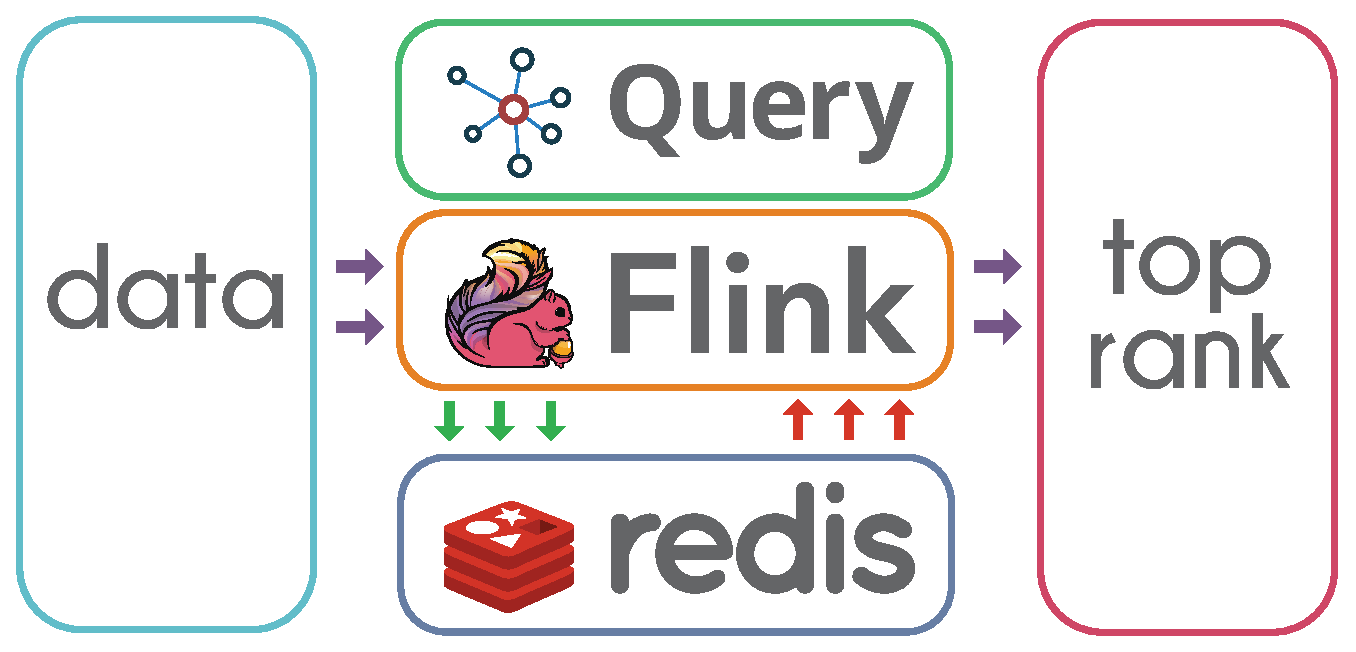
\includegraphics[width=0.35\textwidth]{fig/sostream-layered-architecture.eps}
%	\caption{The layered architecture.}
	\caption{High-level architecture of our solution.}
	\label{fig:sostream-layered-architecture}
\end{figure}

\begin{figure*}[!ht]
	\centering
	\includegraphics[width=.75\textwidth]{fig/query-1-architecture}
	\caption{The topology for Query 1.}
	\label{fig:q1-architecture}
\end{figure*}

The DEBS 2016 Grand Challenge poses two queries that require to efficiently handle several entities interacting each other (i.e., posts and comments) with the goal of discovering some complex dynamics which strongly depend on the passing of time. 
%
The design approach of our application revolves around two principles: parallelization and memory efficiency.
%
The application incorporates two independent solutions that answer the two queries.
%
Aside the specific details, both the solutions %can be easily described 
rely on a sequence of possibly parallel operators that apply stepwise transformations to the incoming events. 
%
Specifically, the application: (1) reads the events from the dataset stored on a file and pushes them within the system;  (2) computes the score associated to each relevant entity (i.e., post, comments); (3) on the basis of this score, determines the top-$k$ rankings with a two-step  approach (being $k$ a query-related parameter); 
and (4) emits the updated top-$k$ rankings. 
%
The meaning of score, and the way it is computed, changes according to the query.
For the first query, each post receives a score resulting from all its comments; the score provided by each comment and the score of the post itself slowly decay with the passing of time. 
%
For the second query, each comment receives a score depending on the size of the community that interacts with it within a given time window. 
%
Due to the great amount of data, computing the score represents the critical operation; therefore, we exploit parallelism to concurrently determine the score by working on independent partitions of the incoming events. 

To focus our effort on the application logic, we need a high-throughput and scalable stream processing framework.  
%
After having examined several alternatives, such as Storm\footnote{\url{http://storm.apache.org/}} and Spark\footnote{\url{http://spark.apache.org/}}, we have chosen Flink~\cite{Flink}, an open source project maintained by the Apache Software Foundation, because it shows promising performance with respect to other well-known frameworks.
%
Our application leverages some advanced features provided by Flink; the most relevant one is the feedback stream, i.e., a stream towards upstream operators, that we use to optimize the usage of memory by deleting expired posts which cannot compete for the top-$k$ ranking ones.
%
To answer the second query, the application also requires to efficiently store the social graph, which represents the users and their friendship relations, in order to periodically compute and retrieve the largest communities. 
%
We solve this problem through Redis~\cite{Redis},an in-memory data structure store, which avoids the bottleneck given by mass storage I/O. 
%
Figure~\ref{fig:sostream-layered-architecture} depicts a high-level overview of our solution.  

\subsection{Query 1}
\label{sec:solution-q1}

The goal of the first query is to determine the updates of the top-3 (i.e., $k=3$) most influential posts in the social network, that is, those that maintain over time a high rate of interaction via comments. 
The scoring discipline encapsulate this concept, and is computed as follows. 
When a post/comment is created, its initial score is set to $10$ and is then decreased by 1 once a day. The post score is the sum of its value plus the score of every direct and indirect comment rooted in it. Once the score reaches zero, the post expires and does not compete for any ranking.
%
We now describe the operators involved in the first query, whose topology is shown in Figure~\ref{fig:q1-architecture}.  

\begin{figure*}[ht]
	\centering
	\includegraphics[width=.75\textwidth]{fig/query-2-architecture}
	\caption{The topology for Query 2.}
	\label{fig:q2-architecture}
\end{figure*}

The \textit{Event Dispatcher} is a centralized operator that reads in parallel posts and comments from several data sources. It converts each entry in a tuple containing only the fields that are strictly necessary to the following operators. Taking advantage of the ascending events timestamp, it can efficiently carry out the interlacing of events. 
%
Afterwards, the \textit{Comment Mapper} maps each comment to the related post. 
%
Observe that this operator also assigns indirect comments (i.e., comments of a post's comment) to the related post by maintaining in-memory a mapping table that links each post with its comments.
%
Storing this mapping table is challenging because it can potentially grow unlimited, thus saturating the memory. 
%
To handle this situation, we exploit the feedback mechanism, which allows us to store only the mapping of not yet expired posts.
%
The \textit{Post Score Updater} is a parallel operator that receives the streams of posts and comments and updates the post score and number of commenters of the post. 
To preserve the application integrity with parallelism, the incoming streams are partitioned by the post identifier.
%
To synchronize the parallel instances of this operator, so to properly update the scores, the upstream operator \textit{Comment Mapper} broadcasts a \textit{time sync} message when the time associated to posts and comments moves forward.
%
The \textit{Aggregator} is a parallel rolling counting operator that merges the single score updates to produce the total score for each post. 
%
Moreover, this operator is in charge of emitting the \textit{Feedback Stream}.
%
The \textit{Post Rank} defines the partial top-3 ranking of posts handled by its upstreams operators; the ranking is sorted by the post score. 
%
Then, the \textit{Post Rank Merger} merges all the partial rankings into a global one and identifies the top-3 posts that trigger the most activity in the social network. 
%
The latest two operators optimize the sorting operations by
%
(1) reducing the elements to be sorted thanks to the parallelization;
%
(2) pruning the expired posts; and 
%
(3) avoiding to sort the elements that cannot actually generate a ranking update (i.e., elements whose score is less than the lowest in the rankings). 
% 
%
Finally, the \textit{Post Rank Filter} produces an updated result every time the top-3 most active posts change.




\subsection{Query 2}
\label{sec:solution-q2}

The second query focuses on identifying the $ k $ recent comments that are supported by the larger communities.
The value of \textit{k} is provided as parameter, whereas a community is defined as the set of users, friends each other, who have liked that comment. 
% 
The topology of our solution is represented in Figure~\ref{fig:q2-architecture}. 
%
The \textit{Event Dispatcher} is a centralized operator that reads in parallel comments, like events, and friendship events from several data sources and, preserving their timestamp order, sends them downstream.
%
The \textit{Friendships Operator} receives the friendship events and updates the social graph, connecting the users that establish a new friend relation. 
The social graph is stored into Redis, where it is represented with adjacency lists indexed by the user identifier.
%
This representation allows us to efficiently retrieve all the user's friends, that are needed to compute the largest community supporting a comment. 
%
The \textit{Comment Score Updater} receives comments and like events, and computes the score associated to each comment as follows. 
%
From each comment that was created not more than \textit{d} seconds ago, where \textit{d} is an input parameter, the operator extracts the set of users $ U $ that have liked it. 
%
For each user $ u \in U $, the \textit{Comment Score Updater} creates a user-based social graph $ G_u $, containing the user $ u $, his/her friends, and the friends of his/her friends; in $ G_u $ the users are interconnected with respect to their friendships. 
%
Afterwards, for each user-based social graph $ G_u, \forall u \in U $, the operator runs a customized version of the well-known and widely used Bron-Kerbosch algorithm~\cite{BronKerbosch1973} to identify the largest clique $ C_u $ associated to each user.
%
Observe that, at this point, the computed cliques depend only on the user-based social graph (i.e., his/her friendships) and also include users who have not liked the comment. 
Therefore, \textit{Comment Score Updater} removes from each clique $ C_u $ the users who have not liked the comment, thus identifying the largest one as the community that supports the comment.
%
Determining the cliques within a graph is an NP-hard problem, so we adopted a lazy approach that executes the Bron-Kerbosch algorithm 
(1) on subgraphs of the social network that, relying on friendships and being independent from like events, should change slowly; and
(2) just on comments that have received a new like event, i.e., avoiding to recompute the clique if not needed.
%
Nevertheless, when a new friendship relation is established, the \textit{Comment Score Updater} invalidates and recomputes all the cliques.
%
Since this operator performs critical operations, we deploy multiple instances of it; to preserve the application integrity while increasing the parallelism, the incoming streams are partitioned relying on the comment identifier.
%
Similarly to the first query, i.e., using a step-wise approach, the \textit{Comment Score Rank} and the \textit{Comment Rank Merger} rank the comments and identify the top-$ k $ ones that are supported by the larger communities.



\section{Evaluation}
\label{sec:evaluation}

In this Section, we present our experimental results.
First, we show the results about the randomness degree of the adopted pseudo-random number generator.
Then, we show the results about the performance recorded by the simulation of the target system.

% %
% EXPERIMENTAL ENVIRONMENT
% %
The experiments have been conducted on an Amazon EC2 c3.8xlarge instance, which is really indicated for high performance science and engineering applications\footnote{https://aws.amazon.com/ec2/instance-types/}.
The instance is equipped with 32 vCPU based on an Intel Xeon E5-2680 v2 (Ivy Bridge) processor, 30 GB of RAM and SSD with 900 IOPS.
It runs Debian 8.3 (Jessie), Python 3.5.2, and the Python-ported version of the official Leemis library for discrete-event simulation, indicated in \cite{leemis2006discrete}.
Our solution has been developed in Python, following the de-facto standard best-practices, stated in \cite{reitz2016,GooglePythonStyleguide}.

% %
% RANDOMNESS ANALYSIS
% %
\subsection{Randomness Analysis}
\label{sec:evaluation-randomness-analysis}
Let us now consider the results about the randomness degree of the adopted generator.
The randomness has been assessed by the following tests:

\begin{itemize}
	\item \textbf{Spectral Test:} this test is considered one of the most powerful tests to assess the quality of linear congruential generators \cite{knuth1981art}. It relies on the fact that the output of such generators form lines or hyperplanes when plotted on 2 or more dimensions. The less the distance between these lines or planes, the better the generator is. In fact, a smaller distance between lines or planes highlights a better uniform distribution.
	
	In Figure~\ref{fig:experimental-analysis-randomness-spectral-16807,fig:experimental-analysis-randomness-spectral-48271,fig:experimental-analysis-randomness-spectral-58012} we show the test results for generators $(16807,2^{31}-1)$, $(48271,2^{31}-1)$ and $(50812,2^{31}-1)$, respectively.
	
	The results show that our generator $(50812,2^{31}-1)$ is much better than $(16807, 2^{31}-1)$, which was a past de-facto standard, and it is really similar to $(48271,2^{31}-1)$, which is the current de-facto standard, according to \cite{leemis2006discrete}.
	
	\item \textbf{Test of Extremes:} this test relies on the fact that if $U=U_{0},...,U_{d-1}$ is an independent identically distributed sequence of $Uniform(0,1)$ random variables, then $\max(U)^{d}$ is also a $Uniform(0,1)$. The test leverages this property to measures, for every stream, how much the generated random values differ from the theoretical uniform distribution.
	
	Given a number of streams $s$ and a level of confidence $c=1-\alpha$, the more the total number of fails is close to the expected value, i.e. $s \cdot c$, the better the generator is.
	
	In Figure~\ref{fig:experimental-analysis-randomness-extremes-50812} we show the test results for the proposed generator $(508012,2^{31}-1, 256)$ with sample size $n=10000$, $k=1000$ bins, sequence size $d=5$ and $95\%$ level of confidence.
	%	
	The proposed generator shows critical values $v_{min}=913$ and $v_{max}=1088$ and 14 total fails (7 lower fails and 7 upper fails), that is not far from the theoretical accepted number of fails, i.e. $256*0.05=13$.
	The proposed generator successfully passed the test with a $94.531\%$ level of confidence.
	
	\item \textbf{Kolmogorov-Smirnov Analysis:} the test measures, at a given level of confidence, the biggest vertical distance between the theoretical cumulative distribution function and the empirical cumulative distribution function.
	The more the recorded distance $d$ is less than the critical value $d*$ for the considered level of confidence, the better the generator is.
	As the Kolmogorov-Smirnov analysis relies on pre-calculated randomness statistics, we have chosen to take into account the statistics obtained by the previous test.
	
	In Figure~\ref{fig:evaluation-randomness-kolmogorov-smirnov-50812} we show the test results for the proposed generator $(50812,2^{31}-1, 256)$ with a $95\%$ level of confidence.
	%
	The proposed generator successfully passed the test, as $d=0.041<0.081=d*$.
	
\end{itemize}

\begin{figure}
	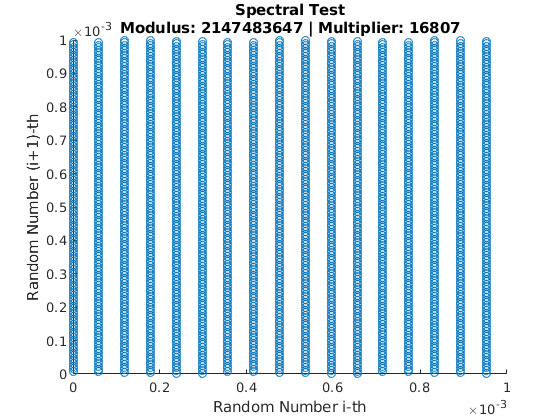
\includegraphics[width=\columnwidth]{fig/evaluation-randomness-spectral-16807}
	\caption{The Spectral Test to evaluate the randomness of the random number generator $(16807,2^{31}-1, 1)$ in the interval $(0, 10^{-3})$.}
	\label{fig:evaluation-randomness-spectral-16807}
\end{figure}

\begin{figure}
	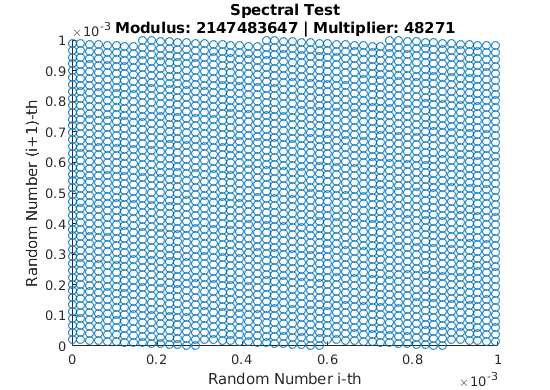
\includegraphics[width=\columnwidth]{fig/evaluation-randomness-spectral-48271}
	\caption{The Spectral Test to evaluate the randomness of the random number generator $(48271,2^{31}-1, 1)$ in the interval $(0, 10^{-3})$.}
	\label{fig:evaluation-randomness-spectral-48271}
\end{figure}

\begin{figure}
	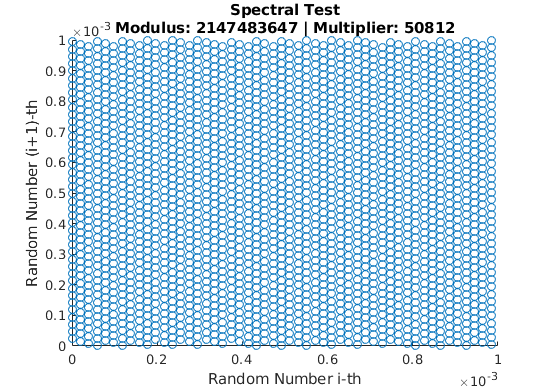
\includegraphics[width=\columnwidth]{fig/evaluation-randomness-spectral-50812}
	\caption{The Spectral Test to evaluate the randomness of the random number generator $(50812,2^{31}-1, 1)$ in the interval $(0, 10^{-3})$.}
	\label{fig:evaluation-randomness-spectral-50812}
\end{figure}

\begin{figure}
	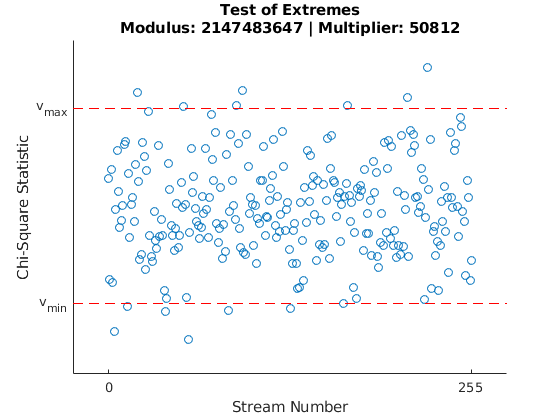
\includegraphics[width=\columnwidth]{fig/evaluation-randomness-extremes-50812}
	\caption{The Test of Extremes with $d=5$ to evaluate the randomness of the random number generator $(50812,2^{31}-1, 256)$.}
	\label{fig:evaluation-randomness-extremes-50812}
\end{figure}

\begin{figure}
	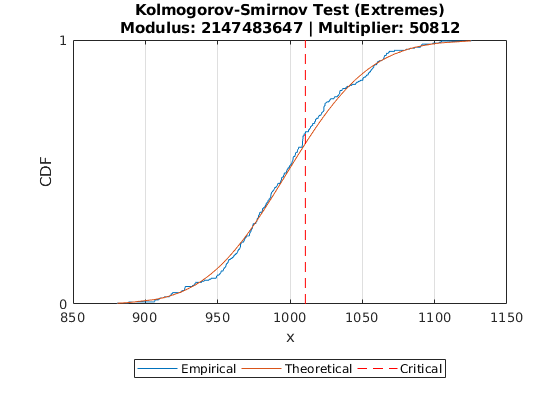
\includegraphics[width=\columnwidth]{fig/evaluation-randomness-kolmogorov-smirnov-50812}
	\caption{The Kolmogorov-Smirnov Analysis (leveraging the Test of Extremes with $d=5$) to evaluate the randomness of the random number generator $(50812,2^{31}-1, 256)$ with $0.95$ confidence level.}
	\label{fig:evaluation-randomness-kolmogorov-smirnov-50812}
\end{figure}


% %
% PERFORMANCE ANALYSIS
% %
\subsection{Performance Analysis}
Let us now consider the experimental results about system performance recorded by our simulator.
In all experiments we considered values stated in Section~\ref{sec:performance-modeling} with a preemption policy based on \textit{random selection}.

\subsection{Transient Analysis}
\label{sec:evaluation-transient-analysis}
First, we conduct a \textit{transient analysis} to evaluate the system stationary in order to (i) prove its convergence to the steady-state and (ii) estimate the duration of the transient period.
%
In fact, given a system that converges to stationary, the knowledge of the duration of the transient period is really important to conduct an effective performance evaluation. In particular, it allows the analyst to focus performance evaluation on a system in its stationary conditions.
%
In the transient analysis we focus on the global system throughput as it can be considered a good representation of the dependency of the system from the initial state.

The following results have been produced by considering an ensemble of $5$ replications, where the $i+1$-th replication is initialized with the last seed of the $i$-th replication, so as to achieve the best decoupling between random sequences of different replications.

In Figure \ref{fig:evaluation-transient-analysis-throughput} we show the transient analysis of the global throughput in the whole system.

The results show that the system reaches the steady-state.
This result is not surprising, because the presence of a stabilizing \textit{infinite-buffer centre}, i.e. the Cloud, largely compensates the possible instability of the \textit{thresholded finite-buffer centre}, i.e. the Cloudlet.

\begin{figure}
	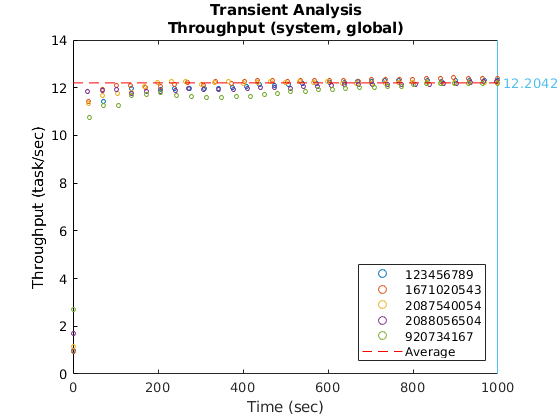
\includegraphics[width=\columnwidth]{fig/evaluation-transient-analysis-throughput}
	\caption{Transient analysis for global throughput in the whole system.}
	\label{fig:evaluation-transient-analysis-throughput}
\end{figure}


\subsection{Performance Evaluation}
Let us now focus on the \textit{performance evaluation}, taking into account the following metrics:

\begin{enumerate}
	\item \textit{response time} both global and classed, both for the system as a whole and for each subsystem;
	
	\item \textit{throughput} both global and classed, both for the system as a whole and for each subsystem;
	
	\item \textit{population} both global and classed, both for the system as a whole and for each subsystem;
	
	\item \textit{interrupted ratio} for tasks belonging to the $2^{nd}$ class.
	
	\item \textit{interrupted response time} for tasks belonging to the $2^{nd}$ class.
\end{enumerate}

In our experiment we assume $S=N=20$, $k=64$ batches, batch dimension $b=512$ and initial seed $iseed=123456789$.
%
Theoretical results have been computed using the formulas presented in Section~\ref{sec:performance-modeling}, assuming the experimentally computed value $E[T_{clt,2,lost}]=1.47445;s.$.

In Table

\begin{figure}
	\begin{center}
		\begin{tabular}{|c||c|c|}
			\hline
			Measure & Theoretical & Experimental\\
			\hline
			$a_{clt,1}$  & $0.978326334857105$ & $0.97911346521$ \\
			$a_{clt_2}$  & $0.603529764734761$ & $0.60502880468$ \\
			$r$          & $0.183573830264005$ & $0.15525744148$ \\	
			\hline
		\end{tabular}
	\end{center}
	\caption{Routing probabilities: comparison between the theoretical result, computed with the analytical model, and the experimental result, computed leveraging our simulator.}
	\label{tbl:evaluation-routing-probabilities}
\end{figure}

\begin{figure}
	\begin{center}
		\begin{tabular}{|c||c|c|}
			\hline
			Measure & Theoretical & Experimental\\
			\hline
			$E[N_{clt}]$  & $123456789$ & $123456789\pm 0.00342$ \\
			$E[N_{clt,1}]$  & $123456789$ & $123456789\pm 0.00342$ \\
			$E[N_{clt,2}]$  & $123456789$ & $123456789\pm 0.00342$ \\
			$E[T_{clt}]$  & $123456789$ & $123456789\pm 0.00342$ \\
			$E[T_{clt,1}]$  & $123456789$ & $123456789\pm 0.00342$ \\
			$E[T_{clt,2}]$  & $123456789$ & $123456789\pm 0.00342$ \\
			$X_{clt}$  & $123456789$ & $123456789\pm 0.00342$ \\
			$X_{clt,1}$  & $123456789$ & $123456789\pm 0.00342$ \\
			$X_{clt,2}$  & $123456789$ & $123456789\pm 0.00342$ \\
			\hline
			$E[N_{cld}]$  & $123456789$ & $123456789\pm 0.00342$ \\
			$E[N_{cld,1}]$  & $123456789$ & $123456789\pm 0.00342$ \\
			$E[N_{cld,2}]$  & $123456789$ & $123456789\pm 0.00342$ \\
			$E[T_{cld}]$  & $123456789$ & $123456789\pm 0.00342$ \\
			$E[T_{cld,1}]$  & $123456789$ & $123456789\pm 0.00342$ \\
			$E[T_{cld,2}]$  & $123456789$ & $123456789\pm 0.00342$ \\
			$X_{cld}$  & $123456789$ & $123456789\pm 0.00342$ \\
			$X_{cld,1}$  & $123456789$ & $123456789\pm 0.00342$ \\
			$X_{cld,2}$  & $123456789$ & $123456789\pm 0.00342$ \\
			\hline
			$E[N_{sys}]$  & $123456789$ & $123456789\pm 0.00342$ \\
			$E[N_{sys,1}]$  & $123456789$ & $123456789\pm 0.00342$ \\
			$E[N_{sys,2}]$  & $123456789$ & $123456789\pm 0.00342$ \\
			$E[T_{sys}]$  & $123456789$ & $123456789\pm 0.00342$ \\
			$E[T_{sys,1}]$  & $123456789$ & $123456789\pm 0.00342$ \\
			$E[T_{sys,2}]$  & $123456789$ & $123456789\pm 0.00342$ \\
			$X_{sys}$  & $123456789$ & $123456789\pm 0.00342$ \\
			$X_{sys,1}$  & $123456789$ & $123456789\pm 0.00342$ \\
			$X_{sys,2}$  & $123456789$ & $123456789\pm 0.00342$ \\
			\hline
			$E[T_{restarted}]$  & $123456789$ & $123456789\pm 0.00342$ \\
			$RestartRatio$  & $123456789$ & $123456789\pm 0.00342$ \\			
			\hline
		\end{tabular}
	\end{center}
	\caption{Performance metrics: comparison between the theoretical result, computed with the analytical model, and the experimental result with level of confidence $95\%$, computed leveraging our simulator.}
	\label{tbl:evaluation-performance-metrics}
\end{figure}

%%
% DISTRIBUTION ANALYSIS
%%
\subsection{Distribution Analysis}
\label{sec:evaluation-distribution-analysis}
In this Section we show the distribution analysis of the Cloudlet global throughput. 
In particular, we focus on both (i) the Probability Density Function (PDF) estimation leveraging distribution fitting, and (ii) the comparison between theoretical and experimental Cumulative Distribution Function (CDF).

In Figure~\ref{fig:evaluation-distribution-analysis-pdf-throughput-cloudlet-global} and  Figure~\ref{fig:evaluation-distribution-analysis-cdf-throughput-cloudlet-global} we show the PDF estimation and the CDF analysis, respectively, for the global Cloudlet throughput when $S=N=20$, where we adopted the \textit{Freedman-Diaconis Rule} for the binning schema.
Results show that the best fitting is the \textit{Normal Distribution} with parameters $\mu\approx7.403$ and $\sigma\approx0.364$.
%
The Normal behavior shown here can be considered as a further good proof of both the system stationary and the effectiveness of the batch means as a tool to study steady-state statistics.

\begin{figure}
	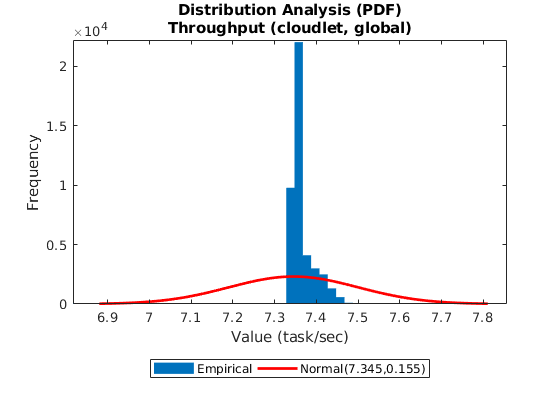
\includegraphics[width=\columnwidth]{fig/evaluation-distribution-analysis-pdf-throughput-cloudlet-global}
	\caption{Distribution analysis (Probability Distribution Function)for the Cloudlet global throughput with threshold $S=N=20$.}
	\label{fig:evaluation-distribution-analysis-pdf-throughput-cloudlet-global}
\end{figure}

\begin{figure}
	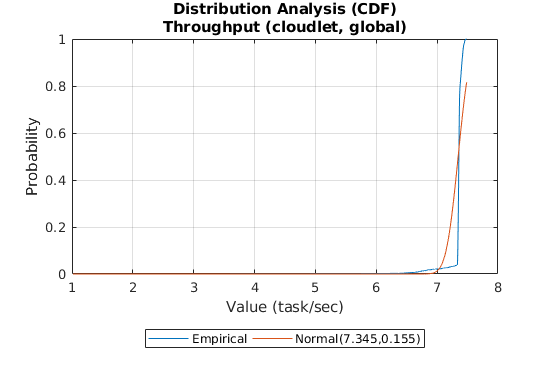
\includegraphics[width=\columnwidth]{fig/evaluation-distribution-analysis-cdf-throughput-cloudlet-global}
	\caption{Distribution analysis (Cumulative Distribution Function) for the Cloudlet global throughput with threshold $S=N=20$.}
	\label{fig:evaluation-distribution-analysis-cdf-throughput-cloudlet-global}
\end{figure}
\section{Conclusions}
\label{sec:conclusions}

\lipsum[1-3]


%********************************************************************************
% Bibliography
%********************************************************************************

\bibliographystyle{abbrv}
\bibliography{./ref/sostream}

\end{document}
